\section{Forsøgsbeskrivelse}

\subsection{Formål}
Formålet med disse forsøg er at for en forståelse af, hvordan de forskellige kredsløb fungere. Derudover bliver der også dannet en baggrundsviden af, hvordan det teoretiske er i kredsløbet. Måledataenes vær-dier kan senere bruges til, at beregne på de forskellige komponenter i kredsløbet. Ud fra måledataene kan der findes en induktans på spolen, som senere kan benyttes til værdi i Plecs, så vores forsøg beskrivelser også kan simuleres, derudover benyttes måledataene også til, at regne på andre forskellige komponenter. Alt dette findes i afsnittet med beregninger.

\subsubsection{LC serie kredsløb}
%\textbf{LC Serie kredsløb}

Materialer:

\begin{itemize}
\item Generator $(50\, \Omega$ modstand)
\item Kapacitor $( 0,1\, \mu F)$
\item Spole/Inductor $(1600$ vindinger)
\item Oscilloskop
\end{itemize}

Opstilling:

\begin{figure}[H]
\centering
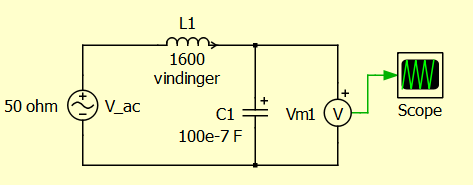
\includegraphics[scale=1]{Vildledning/Schematics/Kredslb/LC_Serie}
\caption{LC Serie Kredsløb}
\label{lcserie}
\end{figure}

Figur \ref{lcserie} viser, hvordan forsøgsopstillingen er bygget op. Forsøget består af en generator, spole og en kapacitor, hvor der sat et oscilloskop til.

\subsubsection{LC parallel kredsløb}

Materialer:

\begin{itemize}
\item Generator $(600\, \Omega$ modstand)
\item Kapacitor $( 0,1\, \mu F)$
\item Spole/Inductor $(1600$ vindinger)
\item Oscilloskop
\end{itemize}

Opstilling:

\begin{figure}[H]
\centering
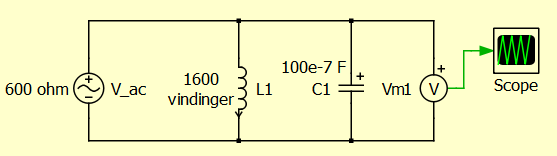
\includegraphics[scale=1]{Vildledning/Schematics/Kredslb/LC_Parallel}
\caption{LC Parallel Kredsløb}
\label{lcparallel}
\end{figure}

Figur \ref{lcparallel} viser forsøgsopstilling af et LC parallel kredsløb, hvor hele kredsløbet sidder parallelt. Kredsløbet er bestående af en generator, en spole og en kapacitor, hvor et oscilloskop er sat til.

\subsubsection{LCR målt over spolen}

Materialer:

\begin{itemize}
\item Generator $(50\, \Omega$ modstand)
\item Kapacitor $( 0,1\, \mu F)$
\item Spole/Inductor $(1600$ vindinger)
\item Modstand/Resistance $(500\, \Omega)$
\item Oscilloskop
\end{itemize}

Opstilling:

\begin{figure}[H]
\centering
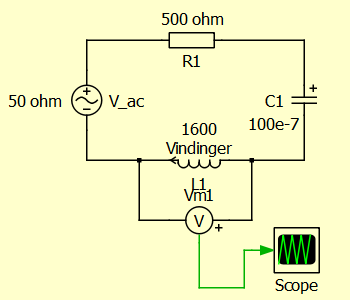
\includegraphics[scale=1]{Vildledning/Schematics/Kredslb/LCR_spole}
\caption{LCR-kredsløb målt over spolen}
\label{lcrspole}
\end{figure}

Figur \ref{lcrspole} viser forsøgsopstilling af et LCR-kredsløb. I dette forsøg bliver der målt over spolen, altså oscilloskopet er sat over spolen. Kredsløbet består af en generator, en spole, en kapacitor og en modstand.

\subsubsection{LCR målt over modstand}

Materialer:

\begin{itemize}
\item Generator $(50\, \Omega$ modstand)
\item Kapacitor $( 0,1\, \mu F)$
\item Spole/Inductor $(1600$ vindinger)
\item Modstand/Resistance $(500\, \Omega)$
\item Oscilloskop
\end{itemize}

Opstilling:

\begin{figure}[H]
\centering
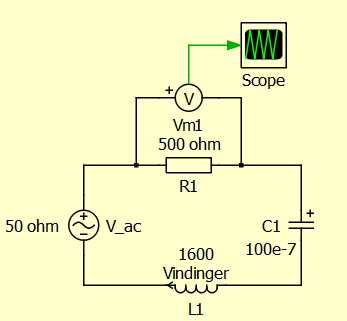
\includegraphics[scale=1]{Vildledning/Schematics/Kredslb/LCR_modstand}
\caption{LCR-kredsløb målt over spolen}
\label{lcrmodstand}
\end{figure}

Figur \ref{lcrmodstand} viser forsøgsopstilling af et LCR-kredsløb. Modsat tidligere forsøg, så bliver der målt over modstanden. Kredsløbet er bestående af samme komponenter som det tidligere forsøg.

\subsection{Fremgangsmåde}

Forsøgende opstilles, 